\newpage

\section{Dynamic Code Optimization}

Most materials are based on \cite{whaley2001partial,stadler2014partial} in this section.

Dynamic compilation systems explore an interesting tradeoff. On one hand, we would like to have code performance
that is comparable to static compilation techniques. However, we would also like to avoid long startup delays, long
latencies, and slow responsiveness, which implies that the
dynamic compiler should be fast.

Many dynamic compilation systems attack this problem by
using an interpreter and an optimizing compiler. They begin
by interpreting the code, and when the execution count for
the method reaches a certain threshold or by some other
heuristic, they use the optimizing compiler to dynamically
compile the code for the method\cite{suganuma2000overview,paleczny2001java} . Some systems
use a fast code generator (baseline compiler) rather than an
interpreter \cite{burke1999jalapeno, cierniak2000practicing}.

The problem with these systems is that the execution speed
of the interpreted or baseline compiled code is significantly
worse than that of fully optimized code — typically 30\% to
ten times slower for baseline compiled code \cite{burke1999jalapeno, cierniak2000practicing} and ten
to a hundred times slower for interpreted code \cite{suganuma2000overview,paleczny2001java}.
Therefore, we would like to transfer into the optimized version as quickly as possible. However, the optimizing compiler can take a long time to compile. Waiting for the optimizing compiler to finish hurts program startup and response times. Some systems use a multi-level compilation
approach, whereby they progress through a number of different compilation “levels”, and thereby slowly “accelerate”
into optimized execution \cite{paleczny2001java,suganuma2001dynamic}. However, this simply
exacerbates the problem of having a long delay until the
program runs at full speed.

Unlike interpretation, compilation takes time that is proportional to the amount of code that is being compiled. Many
analyses and optimizations are superlinear in the size of the
code (basic blocks, instructions, registers, etc.) This can
cause the compilation time to increase significantly as the
amount of code being compiled gets large. Compilation of
large amounts of code is the cause of undesirably long compilation times.


However, when compiling a method at a time, we do not
really have much choice in the matter. Some methods are
large to begin with, and others grow large after performing
inlining. Even when being frugal and inlining only when it
will make a noticeable difference in performance, methods
can still grow large, and excessively restricting inlining can
significantly hurt performance \cite{suganuma2000overview}.


The root of the problem is that method boundaries do not
correspond to the code that would most benefit from optimizing compilation. Even “hot” methods typically contain
some code that is rarely or never executed, but often contain frequently-executed call sites to methods (which in turn,
contain their own rarely-executed code.) Figure \ref{fig:p174} contains a
paraphrased example from the spec db benchmark. In
this example, the \texttt{readdb} method is hot due to the while
loop that it contains. However, the error handling code
guarded by the if and the exception handler are rarely
executed. Likewise, the call to \texttt{read()} is in the loop and
therefore a good candidate for inlining. However, \texttt{read()}
itself contains rarely-executed error handling code. The region that is important to compile — the while loop and the
hot path in \texttt{read()} — have nothing to do with the method
boundaries. Using a method granularity causes the compiler
to waste time compiling and optimizing large pieces of code
that do not matter.


\begin{figure}[H]
	\centering
	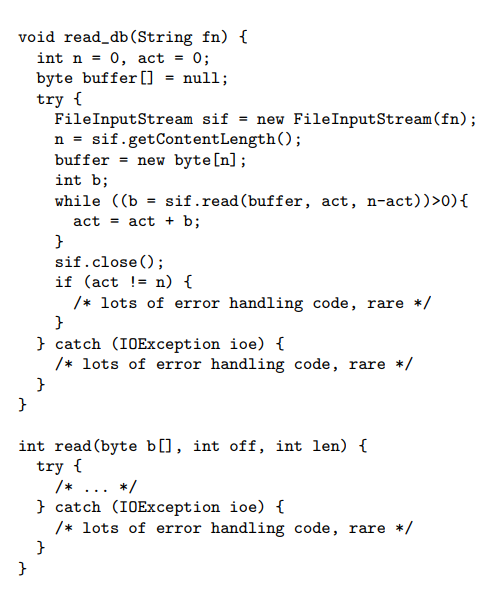
\includegraphics[width=0.5\textwidth]{p174.png}
	\caption{From spec db. Method boundaries do not
		correspond well to where the time is actually spent.}
	\label{fig:p174}
\end{figure}

John Whaley\cite{whaley2001partial} describes a technique to selectively compile and
optimize partial methods. This gives us much better control
over what we spend time compiling and optimizing. This
technique uses dynamic profile data to make a prediction of
what code will actually be executed, and selectively compiles and optimizes only that code. If the program actually
attempts to branch to code that was not compiled (so-called
“rare code”), the system falls back to interpretation or another dynamically compiled version.

\subsection{Partial Method Compilation}


view
The general idea of the technique is to replace all entries
into rare blocks with stubs that transfer control to the interpreter. The rare blocks are completely removed from the
compiler’s intermediate representation. Only very minimal
changes to the compiler are necessary; optimizations can
optionally use rare block information to attempt to better
optimize the common paths. At the end of compilation, we
store a map corresponding to each interpreter transfer point,
which specifies how to reconstruct the interpreter state at
that point.


We now describe each step of the process in detail.


\textbf{1. Based on profile data, determine the set of rare
	blocks.}
The entry points of the rare basic blocks
are mapped to abstract program locations, which then used to mark basic blocks as rare in the compiler’s
intermediate representation.

\textbf{2. Perform live variable analysis.}
Before any transformations are performed, we perform
live variable analysis to determine the set of live variables at rare block entry points.

\begin{figure}[H]
	\centering
	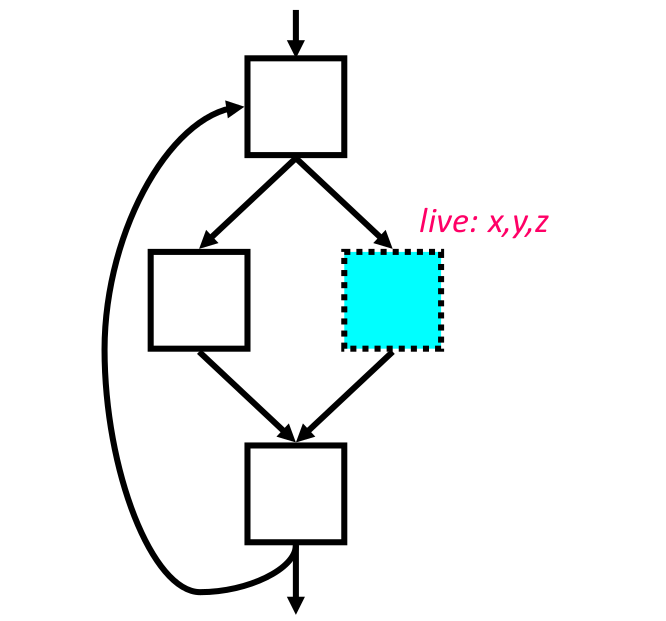
\includegraphics[width=0.3\textwidth]{p176.png}
	\caption{Determine the set of live variables at rare block entry points.}
	\label{fig:p176}
\end{figure}

\textbf{3. Redirect the control flow edges that targeted
	rare blocks, and remove the rare blocks.}
For each control flow edge from a non-rare block to a
rare block, we generate a new basic block containing
a single instruction that transfers control to the interpreter. This instruction uses all local variables and
Java stack locations from the Java bytecode that are
live at that point. We redirect the control flow edge
to point to this new block, and add an edge from the
new block to the exit node. See Figure \ref{fig:p177} for an example. After this process, rare blocks can be removed
as unreachable code.


\begin{figure}[H]
	\centering
	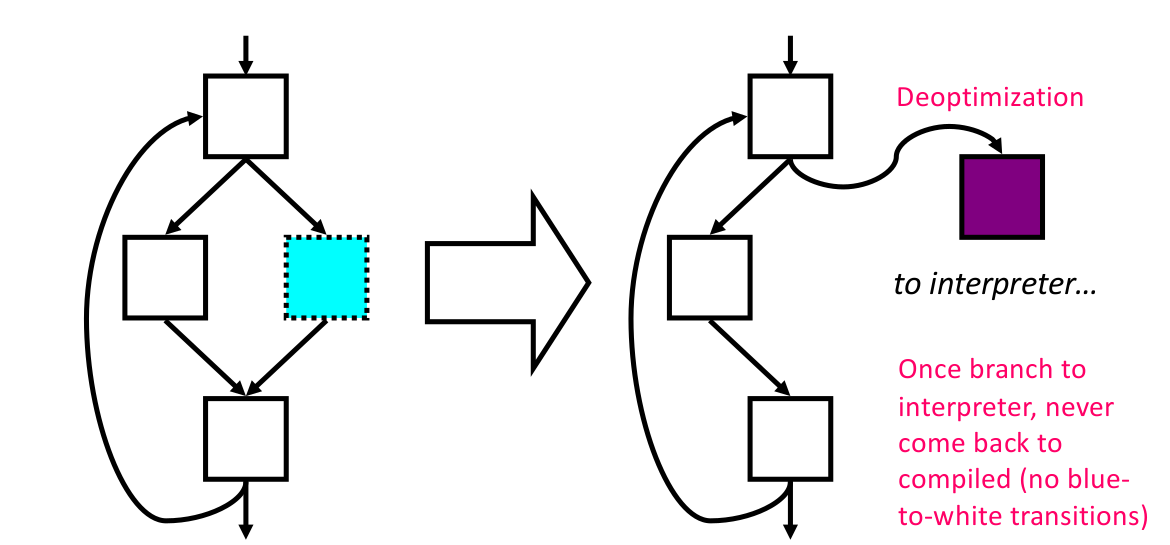
\includegraphics[width=0.5\textwidth]{p177.png}
	\caption{An example of redirecting the rare path.
		On the left, the dotted block is rare, so we redirect
		it to a block that calls the interpreter.}
	\label{fig:p177}
\end{figure}

\textbf{4. Perform compilation normally.}
All analysis, optimization, and code generation proceeds normally. Analyses treat the interpreter transfer
point as an unanalyzable method call.

\begin{figure}[H]
	\centering
	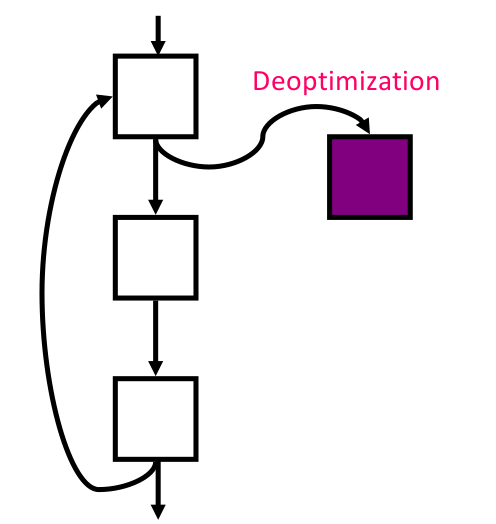
\includegraphics[width=0.3\textwidth]{p178.png}
	\caption{Analyses treat the interpreter transfer point as an unanalyzable method call.}
	\label{fig:p178}
\end{figure}

\textbf{5. Record a map for each interpreter transfer
	point.}
When generating the code to call the glue routine, we
also generate a map that specifies the location, in registers or memory, of each of the local variables and
Java stack locations used in the original Java bytecode.
This map is used by the glue routine to reconstruct the
interpreter state. The map is stored immediately after the call in the instruction stream. Each map is
typically under 100 bytes long.


\begin{figure}[H]
	\centering
	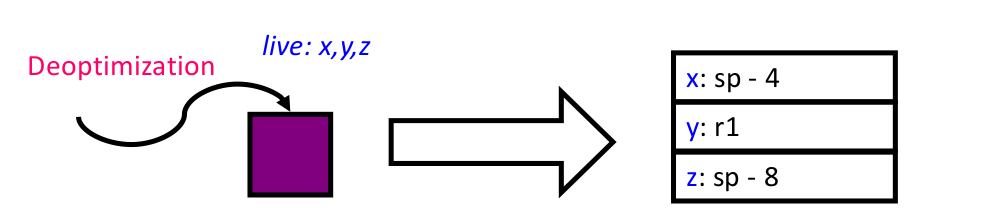
\includegraphics[width=0.5\textwidth]{p179.png}
	\caption{In code generation, generate a map that specifies the location, in registers
		or memory, of each of the live variables used to reconstruct the interpreter state}
	\label{fig:p179}
\end{figure}




\subsection{Partial dead code elimination}

We modified our dead code elimination algorithm to treat
rare blocks specially. This allows us to move computation
that is only live on a rare path into the rare block, saving
computation in the common case.
Our dead code elimination uses an optimistic approach similar to the one described by Muchnick \cite{muchnick1997advanced}, originally due to
Kennedy \cite{kennedy1979survey}. That analysis begins by marking all instructions that compute essential values, and then recursively marking all instructions that contribute to the computation
of essential values. Any non-essential instructions are then
eliminated.

Our analysis operates on SSA form. It first computes the
essential instructions in all non-rare blocks, completely ignoring all rare blocks. An essential instruction computes a
value that is used in a predicate, returned or output by the
method, or has a potential side-effect.
It then visits each
rare block to discover instructions that are essential for that
rare block, but not essential for non-rare blocks. If these
instructions are recomputable at the point of the rare block,
they can be safely copied there.


For each instruction in the rare block, it recursively visits
all instructions that contribute to the computation of values
for that instruction. If an instruction is marked as essential,
it is skipped. If it is a $\Phi$ function, it depends on an earlier
predicate, and is therefore (recursively) marked as essential.
Otherwise, the instruction is added to a set of instructions
associated with the rare block.
After computing sets for all rare blocks, it adds each of the
non-essential instructions in a set to its corresponding rare
block. Then, all instructions in non-rare blocks that are not
marked as essential are eliminated.


Now we make an argument of correctness. Any instruction
that was eliminated on the main path either computed a
value that was not essential anywhere, in which case it is
obviously correct to eliminate it, or it was only essential in
some number of rare blocks, in which case it would have
been copied into those rare blocks. Copying the instruction
into a rare block is legal because, as the instruction is not a $\Phi$
function, the instruction dominates and is in the same loop
as the rare block and therefore would have executed exactly
once. Also, any instruction with a potential side effect or
that read from or wrote to memory would have been marked
as essential on the main path and therefore executed in its
original location. Therefore, moving the instruction to a
rare block does not violate exception or memory semantics.

\begin{figure}[H]
	\centering
	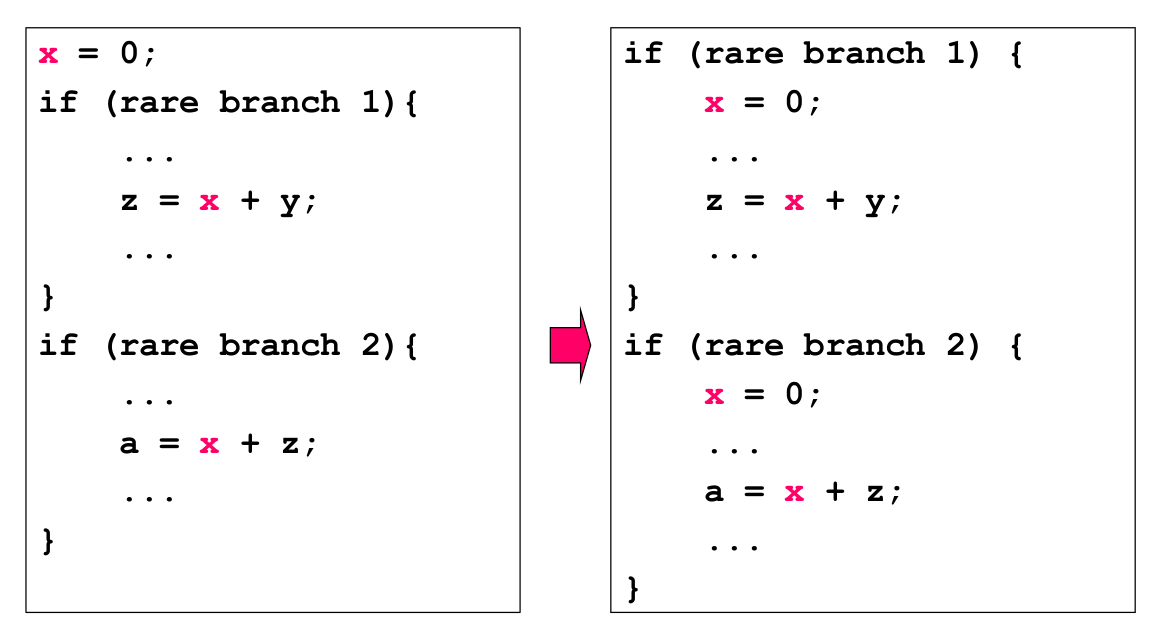
\includegraphics[width=0.6\textwidth]{p180.png}
	\caption{Partial Dead Code Example.}
	\label{fig:p180}
\end{figure}


\subsection{Escape Analysis\cite{stadler2014partial}}

Escape Analysis checks whether an allocated object escapes
(i.e., can be used outside) the allocating method or
thread. This happens, for example, if it is assigned to a
global variable or heap object, or if it is passed as a parameter
to some other method. Compilers use Escape Analysis
to determine the dynamic scope and the lifetime of allocated objects.
The result of this analysis allows the compiler to perform numerous
optimizations on operations such
as object allocations, synchronization primitives and field
accesses.



Figure \ref{fig:p181} shows a small piece of code that will serve as an
example to show the benefits of Escape Analysis:
The \texttt{getValue} method creates a new \texttt{Key} object and checks whether
it is in the cache. If so, the method returns the cached value.
Otherwise, it creates and returns a new value (the method
\texttt{createValue} is not discussed here).

\begin{figure}[H]
	\centering
	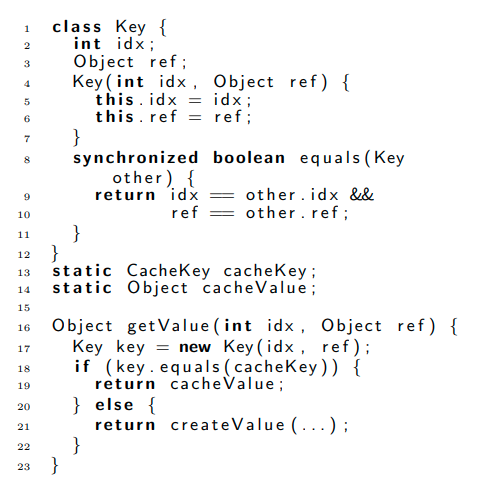
\includegraphics[width=0.6\textwidth]{p181.png}
	\caption{Simple example.}
	\label{fig:p181}
\end{figure}



When \texttt{getValue} is compiled, the compiler will most
likely
perform some inlining, which might cause the actually
compiled code to look like \ref{fig:p182}.
The Key constructor and the
equals method have been inlined into the getValue method,
and a \texttt{synchronized } block was created to achieve synchronization on the inlined equals method.

\begin{figure}[H]
	\centering
	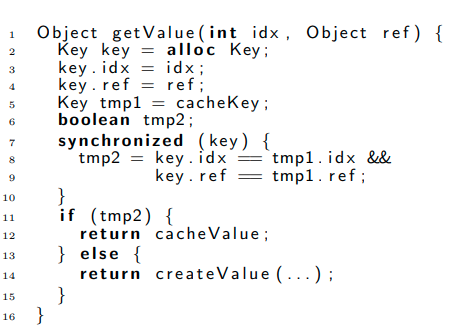
\includegraphics[width=0.6\textwidth]{p182.png}
	\caption{ Example from Figure \ref{fig:p181} after inlining.}
	\label{fig:p182}
\end{figure}


When Escape Analysis examines the resulting method,
it will come to the conclusion that no reference to the
allocated \texttt{Key} object escapes from the
current compilation scope.

This implies that no references to the object exist after the
method has returned, and that no other thread can ever
see a reference to this object. The compiler can use these
observations to perform a number of optimizations:
\begin{itemize}
	\item  The allocation of the object on the garbage collected
	      heap can be replaced with allocation on the stack or
	      in other non-garbage-collected allocation areas such as
	      zones.
	\item Scalar Replacement can be used to eliminate the allocation altogether, by replacing the fields of the object
	      with local variables.
	\item Since the object’s lock will never be contended,Lock
	      Elision can remove the synchronization on \texttt{key}.
\end{itemize}



If the compiler uses Scalar Replacement and Lock Elision,
the result might look like in Figure \ref{fig:p183}.
The allocation was
replaced with the local variables \texttt{idx1} and
\texttt{ref1}, and the
\texttt{synchronized} statement was removed entirely.

\begin{figure}[H]
	\centering
	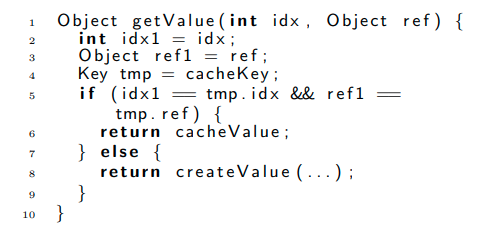
\includegraphics[width=0.6\textwidth]{p183.png}
	\caption{ Example from Figure \ref{fig:p182} after inlining.}
	\label{fig:p183}
\end{figure}

Traditionally, Escape Analysis uses algorithms such as
Equi-Escape Sets \cite{kotzmann2005escape} to determine which objects escape from
the scope. These algorithms build sets of objects that have
the same escape state, with each object initially being in a
separate set. By analyzing all operations in the method the
system can merge sets (e.g., when an object in one set is assigned to a field of an object in another set), or mark a
set as escaping (e.g., when an object in this set is assigned
to a global variable).

\subsection{PARTIAL ESCAPE ANALYSIS}


Escape Analysis allows a compiler to determine whether an
object is accessible outside the allocating method or thread.
This information is used to perform optimizations such as
Scalar Replacement, Stack Allocation and Lock Elision, allowing modern dynamic compilers to remove some of the
abstractions introduced by advanced programming models.







State-of-the-art Virtual Machines employ techniques such
as advanced garbage collection, alias analysis and biased
locking to make working with dynamically allocated objects
as efficient as possible. But even if allocation is cheap, it
still incurs some overhead. Even if alias analysis can remove
most object accesses, some of them cannot be removed. And
although acquiring a biased lock is simple, it is still more
complex than not acquiring a lock at all.

Escape Analysis can be used to determine whether an object needs to be allocated at all, and whether its lock can
ever be contended. This can help the compiler to get rid of
the object’s allocation, using Scalar Replacement to replace
the object’s fields with local variables.

Escape Analysis checks whether an object escapes its allocating method, i.e., whether it is accessible outside this
method. An object escapes, for example, if it is assigned
to a static field, if it is passed as an argument to another
method, or if it is returned by a method. In these cases the
object needs to exist on the heap, because it will be accessed
as an object in some other context.

In many cases, however, an object escapes just in a single
unlikely branch. Nevertheless, this prevents optimizations.
Therefore, we suggest a flow-sensitive Escape Analysis which
we call Partial Escape Analysis.

The idea behind Partial Escape Analysis is to perform optimizations such as Scalar Replacement in branches where
the object does not escape, and make sure that the object
exists in the heap in branches where it does escape.


In many cases, making a global decision about the escapability of objects does not allow the compiler to perform the
above optimizations. For example, the object allocated in
Figure \ref{fig:p184}  escapes into the global variable \texttt{cacheKey}, so that
Escape Analysis would consider it to be escaping.
\begin{figure}[H]
	\centering
	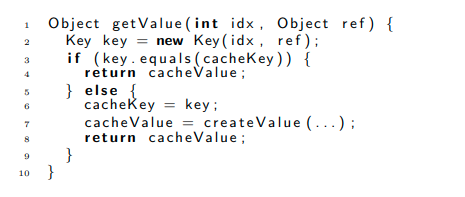
\includegraphics[width=0.6\textwidth]{p184.png}
	\caption{Complex example.}
	\label{fig:p184}
\end{figure}

However, if we only consider the path through the true
branch of the if statement, the object does not escape. Analyzing the escapability of objects for individual branches is
called Partial Escape Analysis. Partial Escape Analysis iterates over the code and maintains the current escape state
and the current contents of allocated objects during this
process. Initially, each allocated object is in the state \texttt{virtual}, which means that there was no reason yet to actually
allocate it. As the algorithm progresses along the control
flow, it updates this state when instructions operate on the
allocated object.


The transition from Figure \ref{fig:p185} to Figure \ref{fig:p186} shows how Partial Escape Analysis lets the compiler optimize the code in
this example:

\begin{figure}[H]
	\centering
	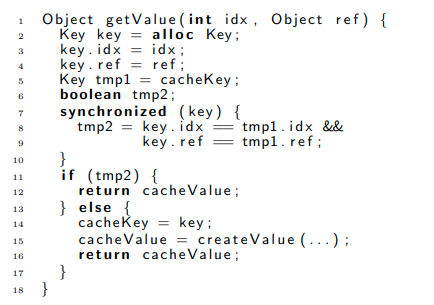
\includegraphics[width=0.6\textwidth]{p185.png}
	\caption{Example from \ref{fig:p184} after inlining.}
	\label{fig:p185}
\end{figure}
\begin{figure}[H]
	\centering
	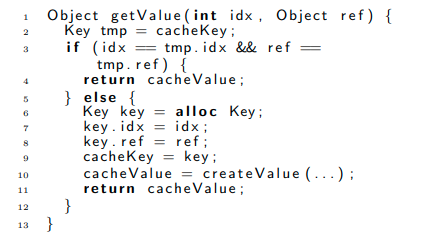
\includegraphics[width=0.6\textwidth]{p186.png}
	\caption{ Example from  \ref{fig:p185} after Partial
		Escape Analysis.}
	\label{fig:p186}
\end{figure}



\begin{itemize}

\item The allocation in line 2 is removed, and an entry for
this object is created that specifies that it is \texttt{virtual}
and that all fields have their default values.
\item The assignments to the fields \texttt{idx} and \texttt{ref }in lines 3
and 4 are removed, and their effects are remembered
by updating the object’s field states.
\item When entering the \texttt{synchronized } region in line 7, the
object is still \texttt{virtual}. The monitor enter operation is
removed, and the object’s state is augmented with a
\texttt{locked } flag that specifies that this object would have
been \texttt{locked } if it actually existed at this point.
\item The accesses to the \texttt{idx} and \texttt{ref }fields of the \texttt{virtual}
object in lines 8 and 9 can be replaced using the object’s current field states.
\item When exiting the \texttt{synchronized } region in line 10, the
object is still \texttt{virtual}. Thus, the monitor exit operation is removed, and the \texttt{locked } flag is removed from
the object’s state.
\item At the \texttt{if} statement in line 11, a copy of the current
state is created, because it has to be propagated to
both successors of this control split.
\item  When continuing at line 12, the object is still \texttt{virtual},
and the return statement ends the processing of this
branch.
\item  When continuing at line 14, the object is still \texttt{virtual},
but the assignment to the static field \texttt{cacheKey} lets
the object escape. In order for it to escape, it needs
to exist, and therefore the object needs to be created
and initialized with the current state of its fields at
this point. This process is called materialization in
our system. The object is transitioned to the state
escaped at this point, and the state of its fields cannot
be used from here on since there could be assignments
to the fields from outside the compilation scope.
\item  Lines 15 and 16 do not affect the state of the object
anymore.
\end{itemize}


In effect, the allocation was moved into one branch of the
if statement. While this did not lead to fewer allocation
sites in the resulting code, it reduces the dynamic number
of allocations at runtime. The actual reduction depends on
the likelihood of the branch containing the allocation being
reached, but there will always be at most as many dynamic
allocations as in the original code.